\chapter{文書検索のための自然言語処理}
本章では文書検索の観点から必要な,自然言語処理の基礎技術について述べる.
まず最初に,文章を単語列にする形態素解析について説明する.
次に自然言語処理において,情報検索に多く使われている特徴量の,TF-IDFについて述べる.
その後,単語の共起頻度を表すPMI(Pointwise Mutual Information)について述べる.
最後に,文書検索の評価尺度の1つであるMAP(Mean Average Precision)について説明する.

\section{形態素解析}
前処理として形態素解析を行う.
形態素とは,「ある言語において,それ以上分解すると意味をなさなくなるところまで分解して抽出された,音素のまとまりの一つ一つ」である.
日本語においては,形態素は単語と同じ意味を持つ.
形態素解析とは,与えられた文字列を形態素の列に分割し,品詞を解析する作業である.
本研究における形態素解析の目的は,単語の出現回数のカウントを可能にし,単語が名詞であるかどうかを判定することにある.
本研究では,形態素解析にMeCab\cite{MeCab}を用いた.

\subsection{MeCab}
MeCabとは, 京都大学情報学研究科-日本電信電話株式会社コミュニケーション科学基礎研究所 共同研究ユニットプロジェクトを通じて開発された
オープンソース 形態素解析エンジンである.
% 言語,辞書,コーパスに依存しない汎用的な設計を基本方針としている.
パラメータの推定にCRF(Conditional Random Fields)を用いており,隠れマルコフモデルを採用している形態素解析器のChaSen\cite{ChaSen}より
精度が向上している.
また,外部から容易に利用できるようなインターフェースを備えているため,他のシステムに組み込みやすいという特徴を持つ.

\section{TF-IDF}
ここでは,現在の情報検索で最も多く使われているTF-IDFについて説明する.
TF-IDFとは,特定文書に頻出し,なおかつ他の文書には出現しにくい語を重要とする手法である.
文書$d$における単語$w$のTF-IDFは,TF(Term Frequency)とIDF(Inverse Document Frequency)を用いて式(\ref{eq_tfidf})で定義される.\\
\begin{equation}
    tfidf(w,d) = tf(w,d) * idf(w)   \label{eq_tfidf}
\end{equation}
\\
TFは文書$d$における単語の出現回数である.
TFは,文書中に何度も繰り返し言及される語は重要であるという仮定に基づいている.
しかし「私」のような,あまりに頻度が高く,どの文書にも出現する語(汎用語)は,文書を特徴付ける上で重要ではないと言える.
この問題の対処のために,IDFを導入する.
IDFは$N$個の文書の集合$D$の中で,単語$w$の出現する文書が少ないほど高い値を取るものである.
汎用語はTFが高くなるが,どの文書にも出現するためにIDFが低くなるため,TF-IDFでは重要語として扱われない.
IDFの計算方法は様々なものがあるが,例えば式(\ref{eq_idf})で計算する.\\
\begin{equation}
    idf(w) = {\rm log} (1 + \frac{N}{df(w)})  \label{eq_idf}
\end{equation}
\\
ここで$df(w)$は,文書集合$D$の中で単語$w$の出現する文書の数を表す.\\

\section{PMI}
本節では,Pointwise Mutual Information(自己相互情報量,PMI)について述べる.
PMIは,2つの事象$X, Y$が存在した時,2事象間の関連の強さを測る尺度であり,式(\ref{eq_pmi})で計算される.
\begin{equation}
    PMI(X, Y) = {\rm log} \frac{P(X, Y)}{P(X)P(Y)}    \label{eq_pmi}
\end{equation}
ここで$P(X)$,$P(Y)$はそれぞれ事象$X$,事象$Y$の生起確率,$P(X, Y)$は事象$X, Y$が共に生起する確率を表す.
PMIは事象$X, Y$が共起しやすいほど正の値をとり,独立の場合には0となる.
% TODO:共起の定義を
本研究では,$P(X)$,$P(Y)$をそれぞれ単語$X$,単語$Y$の生起確率,$P(X, Y)$を単語$X$,単語$Y$の共起確率で計算することにより,
2単語間の関連の強さを推定する.
本研究ではPMIを以下の2点に適応する.
\begin{itemize}
    \item 音声認識結果中の認識誤り単語を推定し,棄却する.
    % TODO:文書検索の話を書く.
    \item クエリや検索対象文書から計算したTF-IDFベクトルの類似度を比較する.
\end{itemize}

\subsection{PMIの計算}
% 式(\ref{equ4.1})における$P(X)$,$P(Y)$,$P(X, Y)$は,別途学習コーパスから計算する.
一般に,文章は冒頭から末尾まで,話題(話の中心的内容)が同じであるとは限らない.
% 話の途中で具体例が出てくること,また話題が切り替わることがしばしばあると考えられる.
複数の話題が含まれる文章において単語の共起を学習すると,別の話題に関する語同士の関連が強くなってしまう.
そのため,文書を話題が変わらない程度の小区間(フレーム)に分割することで,一つの話題を含む区間から単語の生起確率,共起確率を計算する.
具体的には図\ref{fig_pmi}のように,フレームサイズを名詞$N$個を含む区間,フレームシフトを名詞$M$個を含む区間とする.\\

\begin{figure}[htbp]
    \begin{center}
        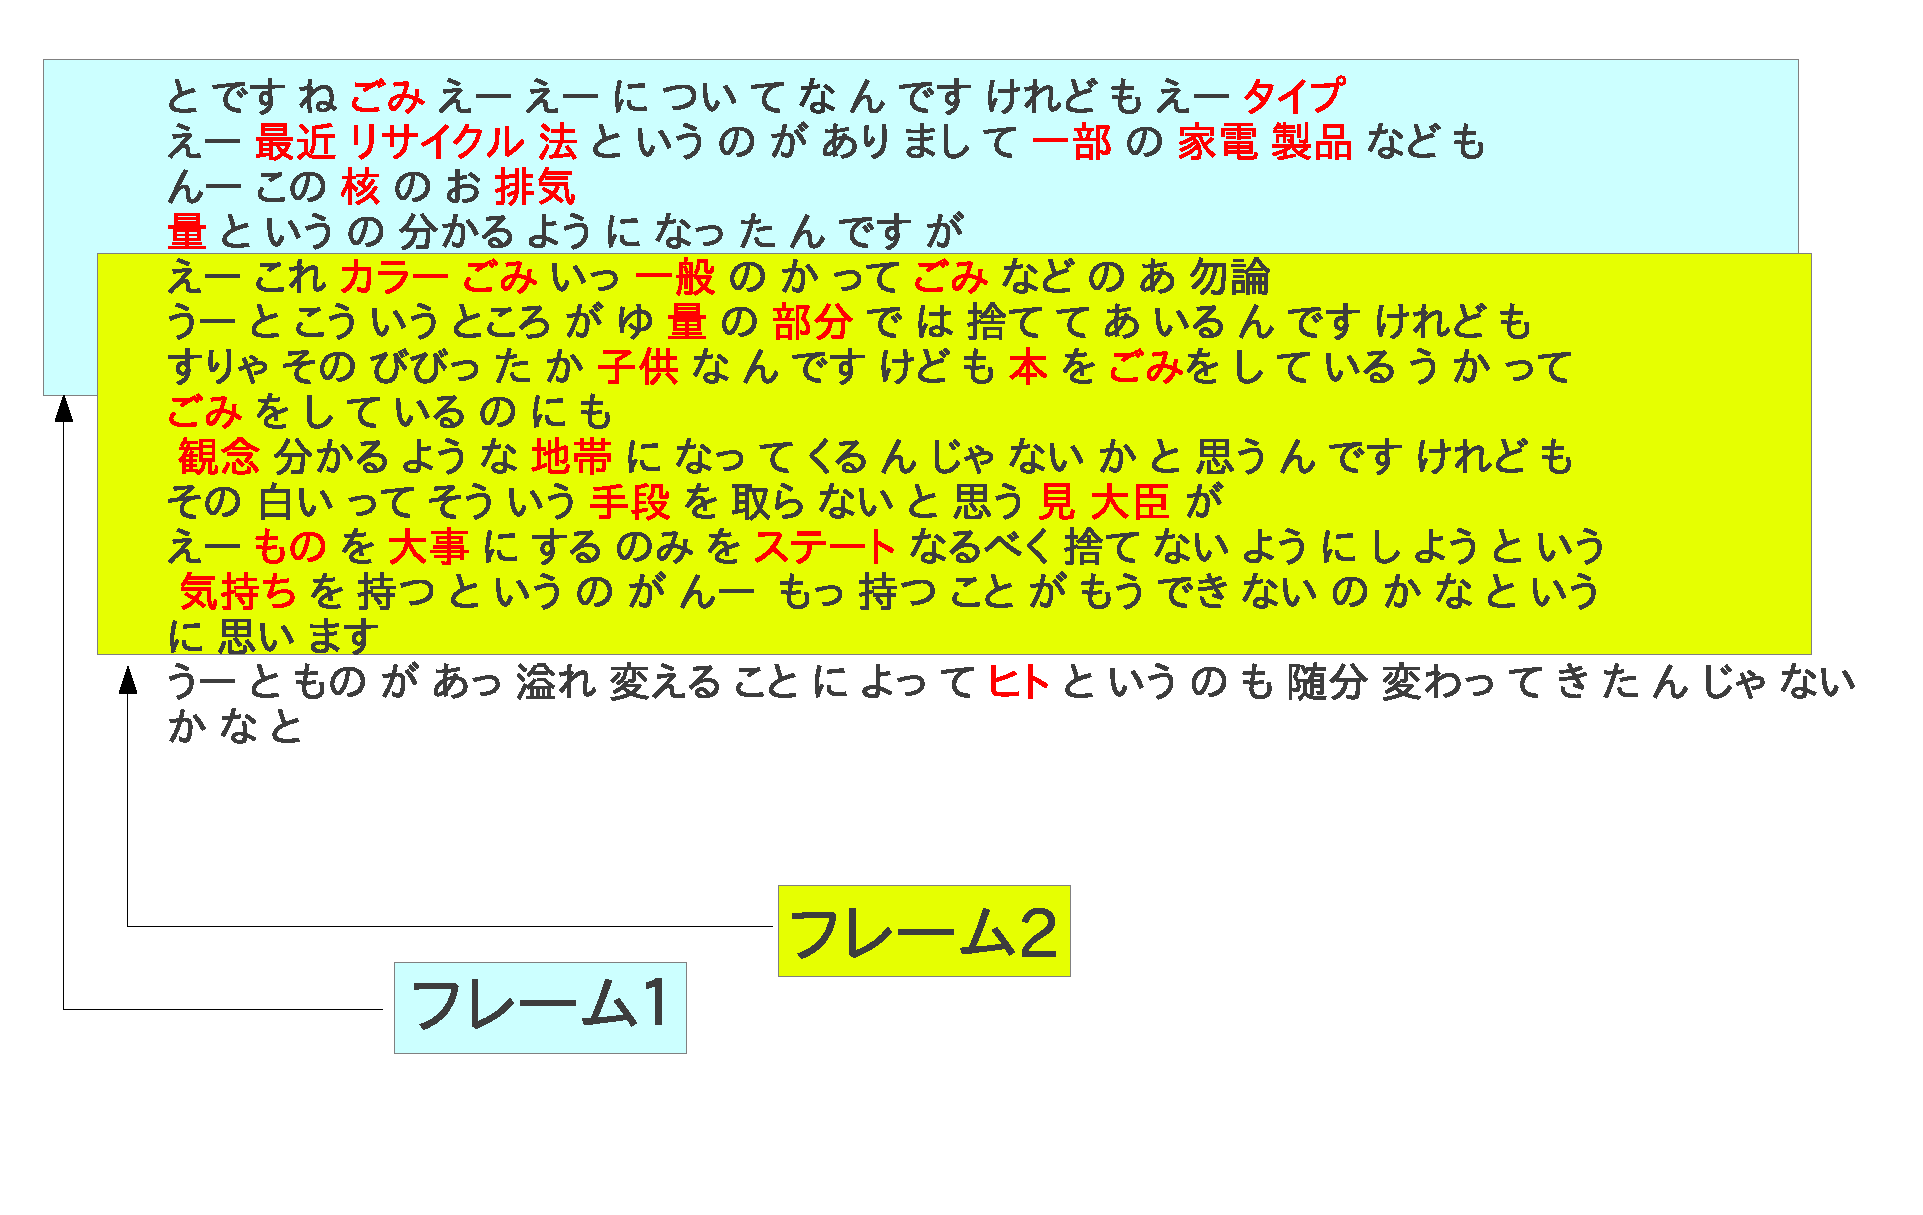
\includegraphics[width=9cm]{framing.eps}
        \caption{フレーム化(N=20, M=10の場合)}
        \label{fig_pmi}
    \end{center}
\end{figure}

式(\ref{eq_pmi})における$P(X)$,$P(Y)$,$P(X, Y)$は,別途学習コーパスから計算する.
学習コーパスが上記のフレーム化によって$K$個のフレームに分割されるとき,$P(X)$, $P(X, Y)$を式(\ref{eq_px})で計算する.\\

\begin{equation}
    P(X) = \frac{f(X)}{K}, P(X, Y) = \frac{f(X, Y)}{K}  \label{eq_px}
\end{equation}
\\
ここで$f(X)$は学習コーパスにおいて単語$X$が出現したフレームの数,$f(X, Y)$は単語$X$と$Y$が共に出現するフレームの数である.

最終的にPMIは,式(\ref{eq_pmi})に式(\ref{eq_px})を代入することにより,式(\ref{eq_pmi2})で求められる.
\begin{eqnarray}
    PMI(X, Y) & = & {\rm log} \frac{\frac{f(X, Y)}{K}}{\frac{f(X)}{K}\frac{f(Y)}{K}}    \nonumber   \\
    & = & {\rm log} \frac{f(X, Y) \cdot K}{f(X)f(Y)}    \label{eq_pmi2}
\end{eqnarray}

\subsection{平滑化PMI}
式(\ref{eq_pmi2})に示した$P(X)$,$P(X, Y)$でPMIを計算する場合,以下の2つの問題がある.
\begin{description}
    \item 問題1 一度も共起しない単語ペアの関連度が測れない. \mbox{} \\
%         $f(x, y) = 0$のとき,$PMI(x, y) = -\infty$となるが,10回ずつしか生起していない単語ペアが共起しなかった場合と,
%         10000回ずつ生起した単語ペアが共起しなかった場合では,後者の方がより共起しにくいと言える.\\
%         10回ずつしか生起していない単語ペアと,10000回ずつ生起した単語ペアが,どちらも共起回数0のときに$PMI(x, y) = \infty$となり,同じ値を取る.
%         しかしながら,10000回ずつ生起した単語ペアのほうが,より共起しにくいと言える.\\
%         $f(X, Y) = 0$のとき,式(\ref{equ4.3})によ$PMI(X, Y) = - \infty$となる.
%         しかし,それぞれ10回ずつしか生起していない2単語が共起しなかった場合と,10000回ずつ生起した2単語が共起しなかった場合では,
%         後者のほうがより関連が弱いはずである.
        $f(x) = f(y) = 10$,$f(x, y) = 0$の単語ペアと,$f(x) = f(y) = 10000$,$f(x, y) = 0$の単語ペアは,式(\ref{eq_pmi2})によれば
        どちらも$PMI(x, y) = -\infty$となり,関連度は同じとなる.しかし信頼性の観点から,前者より後者のほうが関連が弱いとするべきである.
    \item 問題2 低頻度語同士の単語ペアの関連度が過剰に高くなる. \mbox{} \\
        $f(x) = f(y) = f(x, y) = 1$の場合と,$f(x) = f(y) = f(x, y) = 100$の場合では,前者はPMIの値が${\rm log}(K)$,後者は${\rm log}(\frac{K}{100})$
        となり,前者のほうが関連が強いことになる.しかし信頼性の観点から,前者は後者より関連が弱いとするべきである.\\

\end{description}
浅見ら\cite{PMI}によって,これらの問題への対処をした平滑化PMIが提案されている.
問題1に対してはチューリング推定量\cite{turing}を用いて補正し,問題2に対してはt検定によって$P(X, Y)$と$P(X)P(Y)$の差が優位か否かを判定することによって対処する.
平滑化PMIは式(\ref{eq_smoothed_pmi})で定義される.また,式(\ref{eq_smoothed_pmi})中の$\hat{f}(X,Y)$及び${\rm t(X,Y)}$はそれぞれ式(\ref{eq_turing}),式(\ref{eq_t})で計算される.
ここで,$N_0$は学習コーパスで一度も共起しなかった単語ペア数,$N_1$は学習コーパスで一度だけ共起した単語ペア数であり,$\theta$はt検定の閾値である.

\begin{eqnarray}
    PMI(X,Y) &  =  & \left\{
        \begin{array}{ll}
            {\rm log} \frac{\hat{f}(X,Y) \cdot K}{f(X)f(Y)} & {\rm if\ t(X,Y)} > \theta	\\
            0 & {\rm else} \label{eq_smoothed_pmi} \\
        \end{array}
    \right.\\
    \hat{f}(X,Y)  & =  & \left\{
        \begin{array}{ll}
            f(X,Y) & {\rm if}\ f(X,Y) > 0 \\
            \frac{N_1}{N_0} & {\rm else}  \label{eq_turing} \\
        \end{array}
    \right.\\ 
    {\rm t(X,Y)}  & =  & \frac{|\hat{f}(X,Y) - \frac{f(X)f(Y)}{K}|}{\sqrt{\hat{f}(X,Y)}}	\label{eq_t}
\end{eqnarray}

\section{音声文書中の認識誤り単語の棄却手法}
音声認識結果には音声認識誤りが含まれる.これらの認識誤りは,その後の特徴量計算の段階で悪影響を及ぼし,
最終的に文書検索精度を劣化させる原因となる.
本節では音声認識結果から,単語の文脈一貫性の観点から認識誤り単語を推定し,棄却する手法を述べる.
%
% TODO:どこかにベクトル空間モデルに基づく文書比較についての話を

% TODO:卒論からのコピーなので,一部咬み合わない,上と重複する部分がある.

\subsection{単語の文脈一貫性に基づく誤り単語の棄却}  \label{sec_word_rejection}
% TODO:誤り単語が周辺と脈絡なく...要出典,要図
音声認識誤り単語は一般にその周辺の単語と脈絡なく現れ,関連が弱いという特徴がある.
そこで本研究では前述のPMIを用いて,単語と文書の関連度を推定し,関連が弱い語を認識誤り単語として棄却する枠組みを提案する.
文書$d = {w_1, w_2, ..., w_i, ..., w_n}$と,$d$中の単語$w_i$の関連度を,式(\ref{eq_sumpmi})で計算される$sumPMI(w_i)$で推定する.
\begin{equation}
    sumPMI(w_i) = \sum^{n}_{j=1, j \neq i}{PMI(w_i, w_j)}   \label{eq_sumpmi}
\end{equation}
PMIは2単語間の関連の強さを表すため,$sumPMI(w_i)$は単語$w_i$と文書$d$の関連の強さを表すと考えられる.
$sumPMI$が低い語は,文書との関連が弱い語であり,認識誤り単語であることが期待できる.
本研究では,$sumPMI(w)$の値が負となる単語$w$を,認識誤り単語として除外した.

\section{MAP}
SpokenQuery\&Docの評価尺度にはMAP(Mean Average Precision)が用いられている.
これはクエリ毎の平均適合率AP値の平均である.
クエリ$q$に対するAP値$AP(q)$は式(\ref{eq_ap})で計算される.
\begin{equation}
    AP(q) = \frac{1}{|N|} \sum^N_{i=1} \frac{i}{rank(i)}    \label{eq_ap}
\end{equation}
ここで$N$はクエリ$q$に対する正解文書の数,$rank(i)$はクエリ$q$の$i$番目の正解文書が,文書検索によって付けられた順位である.
AP値,MAPは共に[0, 1]の値をとる.
